\documentclass{article}

% if you need to pass options to natbib, use, e.g.:
%     \PassOptionsToPackage{numbers, compress}{natbib}
% before loading neurips_2021

% ready for submission
\usepackage[preprint]{neurips_2021}

% to compile a preprint version, e.g., for submission to arXiv, add add the
% [preprint] option:
%     \usepackage[preprint]{neurips_2021}

% to compile a camera-ready version, add the [final] option, e.g.:
%     \usepackage[final]{neurips_2021}

% to avoid loading the natbib package, add option nonatbib:
%    \usepackage[nonatbib]{neurips_2021}

\usepackage[utf8]{inputenc} % allow utf-8 input
\usepackage[T1]{fontenc}    % use 8-bit T1 fonts
\usepackage{hyperref}       % hyperlinks
\usepackage{url}            % simple URL typesetting
\usepackage{booktabs}       % professional-quality tables
\usepackage{amsfonts}       % blackboard math symbols
\usepackage{nicefrac}       % compact symbols for 1/2, etc.
\usepackage{microtype}      % microtypography
\usepackage{xcolor}         % colors

% proper quoting
\usepackage{csquotes} 

\usepackage{graphicx}

\title{The Effect of Renewable Generation on Electricity Spot Market Prices in Germany}

% The \author macro works with any number of authors. There are two commands
% used to separate the names and addresses of multiple authors: \And and \AND.
%
% Using \And between authors leaves it to LaTeX to determine where to break the
% lines. Using \AND forces a line break at that point. So, if LaTeX puts 3 of 4
% authors names on the first line, and the last on the second line, try using
% \AND instead of \And before the third author name.

\author{%
Ismail Kisa\\
% Matrikelnummer \\
\texttt{ismail.kisa@student.uni-tuebingen.de}\\
\And Gereon Recht\\
% Matrikelnummer \\
\texttt{gereon.recht@student.uni-tuebingen.de} \\
  %David S.~Hippocampus\thanks{Use footnote for providing further information
   % about author (webpage, alternative address)---\emph{not} for acknowledging
   % funding agencies.} \\
  %Department of Computer Science\\
  %Cranberry-Lemon University\\
  %Pittsburgh, PA 15213 \\
  %\texttt{hippo@cs.cranberry-lemon.edu} \\
  % examples of more authors
  % \And
  % Coauthor \\
  % Affiliation \\
  % Address \\
  % \texttt{email} \\
  % \AND
  % Coauthor \\
  % Affiliation \\
  % Address \\
  % \texttt{email} \\
  % \And
  % Coauthor \\
  % Affiliation \\
  % Address \\
  % \texttt{email} \\
  % \And
  % Coauthor \\
  % Affiliation \\
  % Address \\
  % \texttt{email} \\
}

\begin{document}

\maketitle

\begin{abstract}
\begin{itemize}
    \item Increasing renewable generation in Germany $->$ EEG (Erneurbare Energien Gesetz) responsible for that
    \item This paper analyses the effect of renewabele/conventional generation on the spot market price
    \item Analyzed interval from 2019 - 2021
    \item Describe data briefly
    \item We use regression analysis
    \item Mention result: negative correlation of renewable generation and price $->$ merit-order
\end{itemize}


\end{abstract}

\section{Introduction}

\section{Data}
We use hourly time series data published by SMARD (Strommarktdaten) from the federal network agency of germany for our analysis. We analyze hourly data in the period from 2019 to 2021 for electricity generation and the corresponding intraday spot market prices. Originally, the intraday spot market prices are available in 15-minutes intervals. But for our analysis we resampled the spot market prices to hourly intervals using the mean of the respective time slots, to match to the hourly interval of the electricity generation data. SMARD provides the amount of generated electricity that is actually fed into the power grid. The data is clustered into different bidding zones in europe. Since we focuse only on Germany, we use the bidding zone Germany/Luxembourg, which is available from 01.10.2018. Before, Germany was cumulated with Austria and Luxembourg. In a bidding zone, the spot market price is the same everywhere.

\begin{figure}
    \centering
    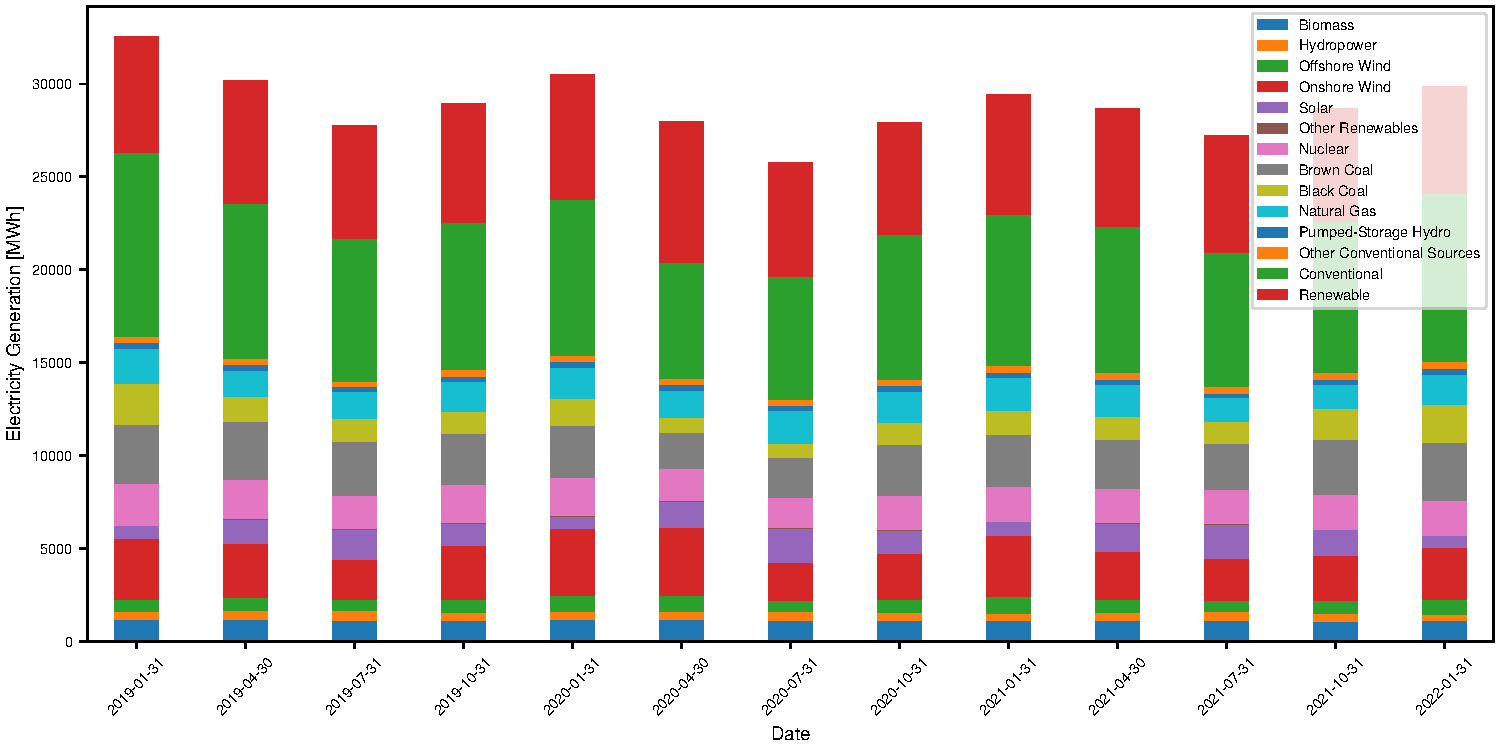
\includegraphics[width=\columnwidth]{doc/fig/quarterly_technology_mix.pdf}
    \caption{Caption}
    \label{fig:quarterly_mix}
\end{figure}

Electricity generation can be divided into two categories: conventional and renewable. Conventional power generation refers to those power plants that require finite, fossil energy resources. These include gas, coal or oil but also nuclear power plants. On the otherside, renwable power generation uses energy sources that are continously renewed and are available unlimited. Examples are hydropower, photovoltaic, wind or biomass. Our data contains, besides the mentioned power plants, "other renewables" and "other conventionals". "Other renewables" include for example geothermal energy or landfill gas. "Other conventionals" incude trash or mineral oil. Those power plants have a small electricity generation and are merged. The most significant energies are wind and solar for renewable, and brown coal and nuclear for conventional. 

The spot market price for electricity is traded on the exchange and is determined by supply and demand. In some hours the price of electricity on the spot market is negative. This happens if high electricity generation meets low demand. In times of negative prices, the electricity generators have to pay for the acceptans of their generated electricity. 

\begin{itemize}
    \item Mention that pumped storage hydro is left out and analyzed seperately?
    \item Mention that the price has increased a lot since 2019, while the percentage of renewable is same?
    \\
    \item Informations from \textit{https://www.smard.de/page/home/wiki-article/446/636, https://www.smard.de/page/home/wiki-article/518/562}
\end{itemize}

\section{Methods}

\section{Results}

\begin{figure}
    \centering
    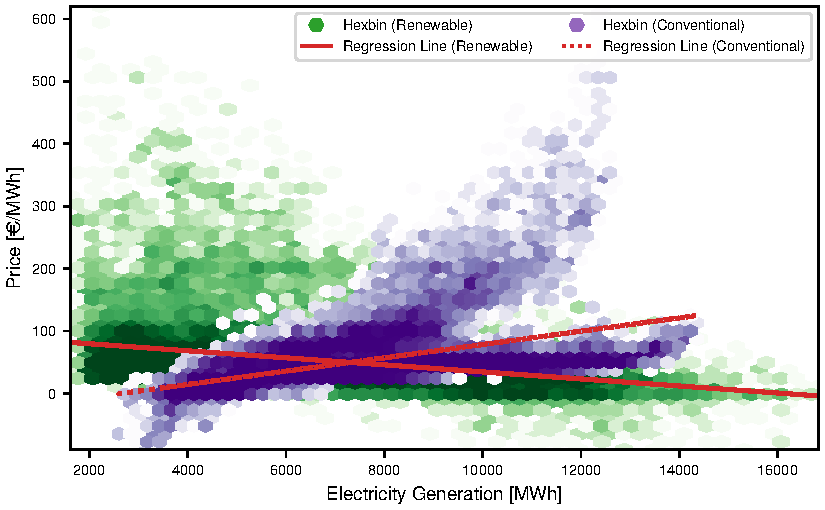
\includegraphics[width=\columnwidth]{doc/fig/ren_vs_con_regression.pdf}
    \caption{Caption}
    \label{fig:ren_vs_con_regression}
\end{figure}

\begin{figure}
    \centering
    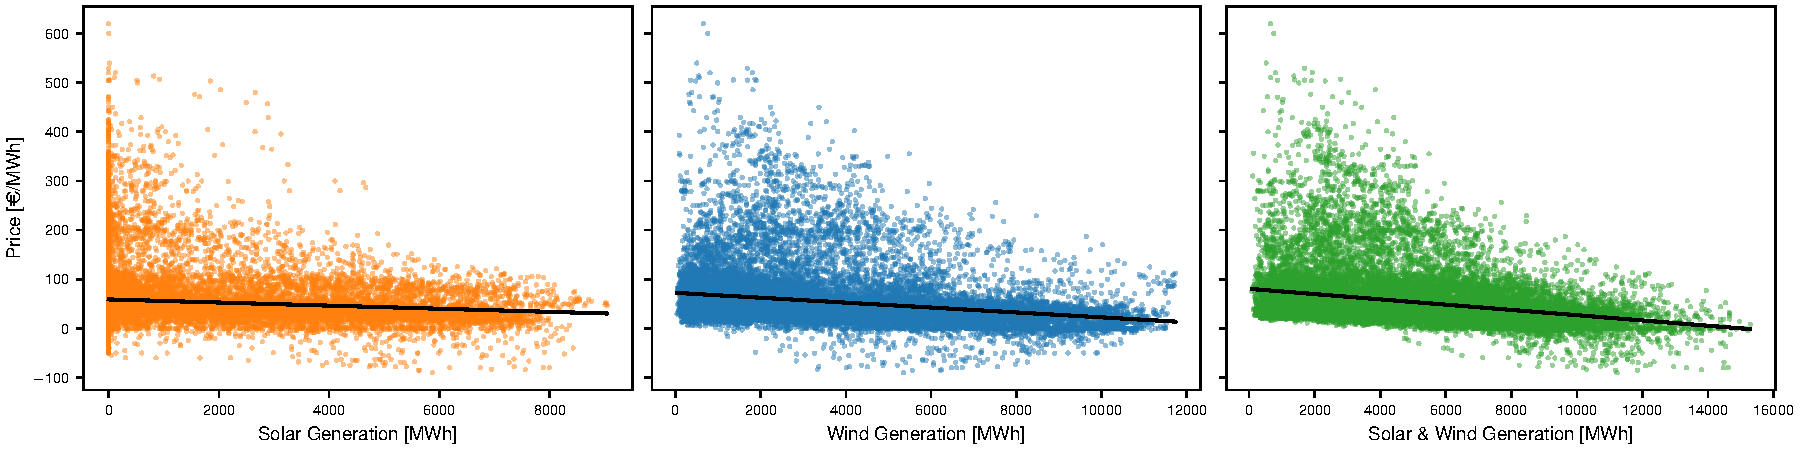
\includegraphics[width=\columnwidth]{doc/fig/solar_wind_regression.pdf}
    \caption{Caption}
    \label{fig:solar_wind_regression}
\end{figure}

\section{Conclusion}


\end{document}
